\documentclass{article}
\title{Analiza algorytmów. Lista 3}
\author{Piotr Berezowski, 236749}

\usepackage{polski}
\usepackage[utf8]{inputenc}
\usepackage{enumerate}
% \usepackage{subfig}
\usepackage{amsmath}
\usepackage{amsfonts}
\usepackage{cleveref}
\usepackage{cases}
\usepackage{mathtools}
\usepackage{float}
\usepackage{graphicx}
\usepackage{caption}
\usepackage{subcaption}
\usepackage[ruled,vlined,linesnumbered,longend]{algorithm2e}
\graphicspath{ {./src/} }

\newenvironment{pseudokod}[1][htb]{
	\renewcommand{\algorithmcfname}{}
	\begin{algorithm}[#1]%
	}{
\end{algorithm}
}

\begin{document}
	\maketitle
	\pagenumbering{gobble}
	\newpage
    \pagenumbering{arabic}
    
    \section{Implementacja zadań}
        Załączone pliki:
        \begin{itemize}
            \item \textit{unique\_sum.go} - zawiera implementację algorytmu przybliżonego sumowania wykożystywanego w zadaniu 9.
            \item \textit{unique\_avg.go} - zawiera implementację algorytmu liczącego średnią unikalnych elementów (zadanie 10).
            \item \textit{generators.go} - zawiera funkcje używane do generowania zbiorów.
            \item \textit{zad1.go, zad2.go} - funkcje generujące dane do wykresów.
            \item \textit{main.go} - zawiera testowane funkcje haszujące i wszystkie funkcje pomocnicze.
            \item \textit{plots.py} - zawiera funkcje rysujące wykresy.
        \end{itemize}
	
	\section{Zadanie 9}
	\subsection{Opis zadania}

        Przeczytaj notatki do wykładu i zaimplementuj opisany tam algorytm przybliżonego sumowania. Wykonaj eksperymenty analogiczne do tych dla przybliżonego zliczania. 
        W szczególności:
        \begin{itemize}
            \item wykorzystaj metodę odwrotnej dystrybuanty i przetestuj różne funkcje haszujące
            \item sprawdź dokładność algorytmu dla różnych scenariuszy, na przykład kiedy wartościcech $\lambda_1, \lambda_2, \dots, \lambda_n$ są takie same, losowo 
                wybrane z rozkładu jednostajnego na przedziale $(a,b)$ dla różnych $a$ i $b$, większość wartości jest podobna ale istnieją wartości odstające
            \item porównaj wyniki eksperymentów z ograniczeniami wynikającymi z nierówności Czebyszewa.
        \end{itemize}
    
    \subsection{Rozwiązanie}

    \subsubsection{Wyniki dla różnych wartości parametru $m$}

        \begin{figure}[H]
            % \centering
            \begin{subfigure}{0.6\textwidth}
                \centering
                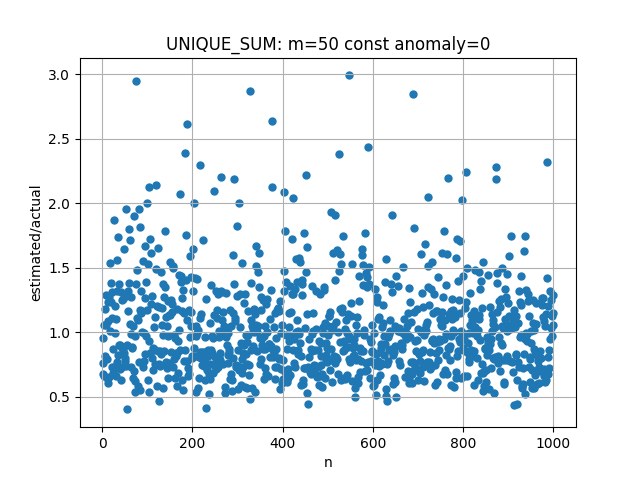
\includegraphics[width=\linewidth]{sum/zad1_m=10.png}
                \caption{m = 10}
            \end{subfigure}
            \begin{subfigure}{0.6\textwidth}
                \centering
                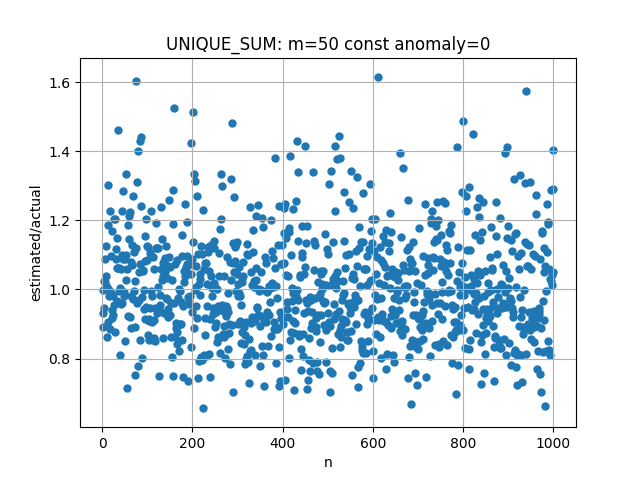
\includegraphics[width=\linewidth]{sum/zad1_m=50.png}
                \caption{m = 50}
            \end{subfigure}
        % \end{figure}
        % \begin{figure}[H]
            \begin{subfigure}{0.6\textwidth}
                \centering
                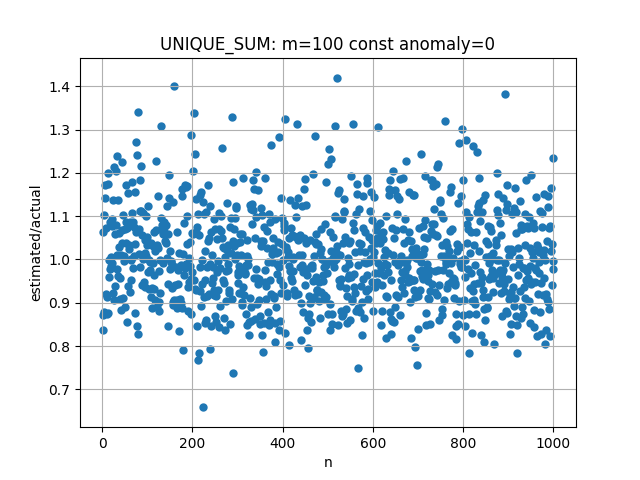
\includegraphics[width=\linewidth]{sum/zad1_m=100.png}
                \caption{m = 100}
            \end{subfigure}
            \begin{subfigure}{0.6\textwidth}
                \centering
                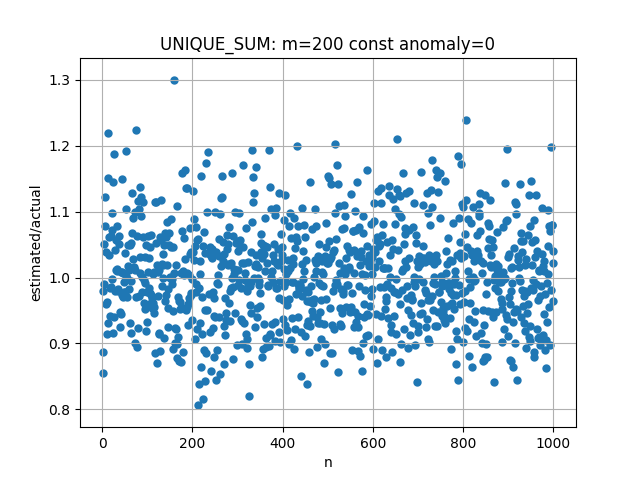
\includegraphics[width=\linewidth]{sum/zad1_m=200.png}
                \caption{m = 200}
            \end{subfigure}
        % \end{figure}
        % \begin{figure}[H]
            \begin{subfigure}{0.6\textwidth}
                \centering
                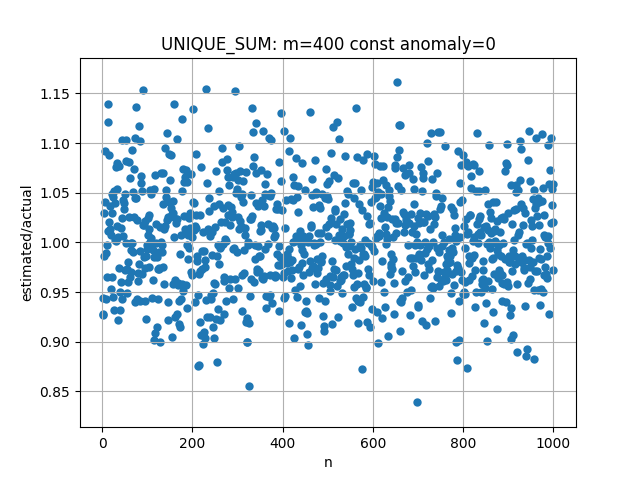
\includegraphics[width=\linewidth]{sum/zad1_m=400.png}
                \caption{m = 400}
            \end{subfigure}
            \begin{subfigure}{0.6\textwidth}
            \end{subfigure}
            \caption{Wykresy dla $\lambda = \textnormal{const}$ i funkcji haszującej $hash1$}
        \end{figure}
    
        Widzimy, że wraz ze wzrostem wartości $m$ rośnie dokładność z jaką szacowana jest suma.

    \subsubsection{Wyniki dla różnych funkcji haszujących}

    \begin{figure}[H]
        \begin{subfigure}{0.6\textwidth}
            \centering
            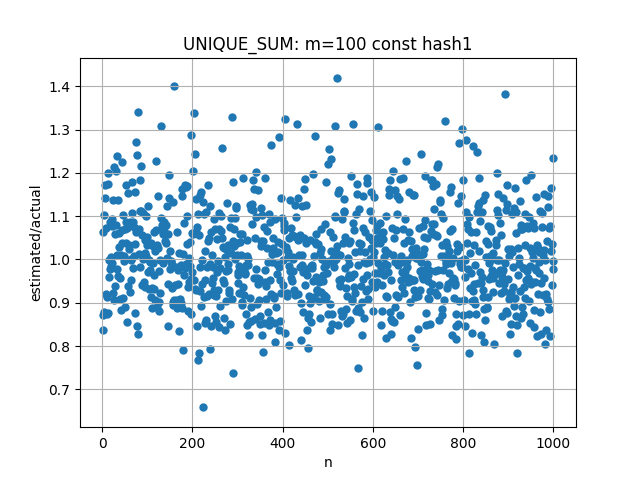
\includegraphics[width=\linewidth]{sum/zad1_hash1_const.png}
            \caption{$h = hash1$}
        \end{subfigure}
        \begin{subfigure}{0.6\textwidth}
            \centering
            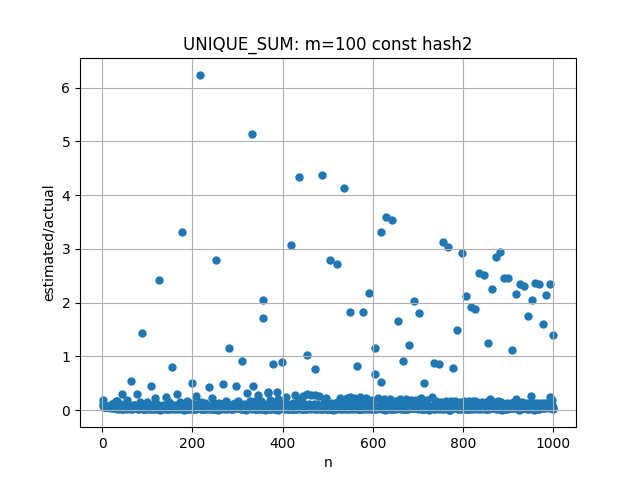
\includegraphics[width=\linewidth]{sum/zad1_hash2_const.png}
            \caption{$h = hash2$}
        \end{subfigure}
        \begin{subfigure}{0.6\textwidth}
            \centering
            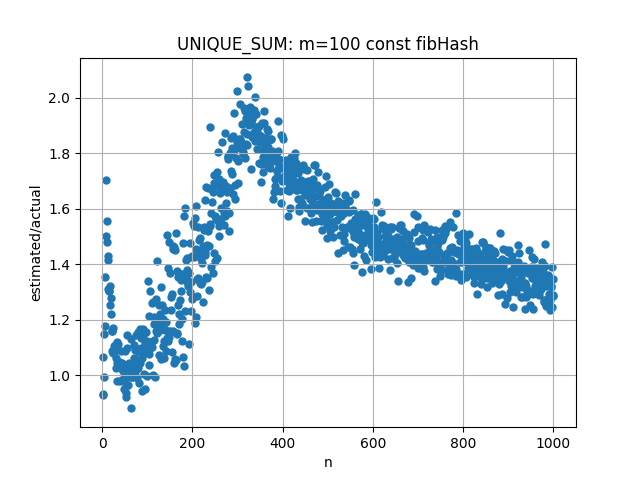
\includegraphics[width=\linewidth]{sum/zad1_fibhash_const.png}
            \caption{$h = fibHash$}
        \end{subfigure}
        \begin{subfigure}{0.6\textwidth}
            \centering
            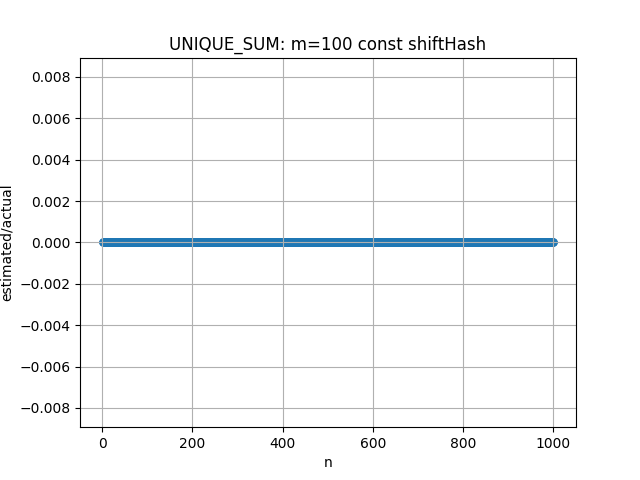
\includegraphics[width=\linewidth]{sum/zad1_shifthash_const.png}
            \caption{$h = shiftHash$}
        \end{subfigure}
        \caption{Różne funkcje haszujące dla wartości $\lambda = \textnormal{const}$ i $m = 100$}
    \end{figure}

    Widzimy, że dla "złych" funkcji haszujących, które są nieodporne na kolizje, lub 
    nierównomiernie "wypełniają" zbiór wartości funkcji estymowana suma była znacznie 
    gorszej jakości niż dla "dobrej" funkcji haszującej jaką jest funkcja etykietowana 
    jako $hash1$.

    \subsubsection{Wyniki dla różnych wartości $\lambda$}

    \begin{figure}[H]
        \begin{subfigure}{0.6\textwidth}
            \centering
            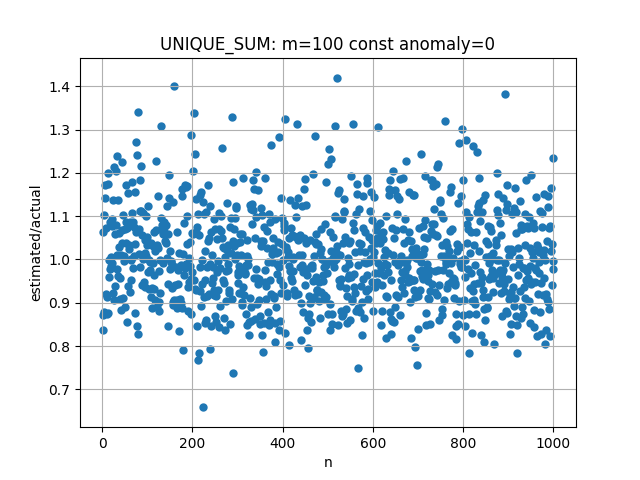
\includegraphics[width=\linewidth]{sum/zad1_const_0.png}
            \caption{$\lambda = \textnormal{const}$}
        \end{subfigure}
        \begin{subfigure}{0.6\textwidth}
            \centering
            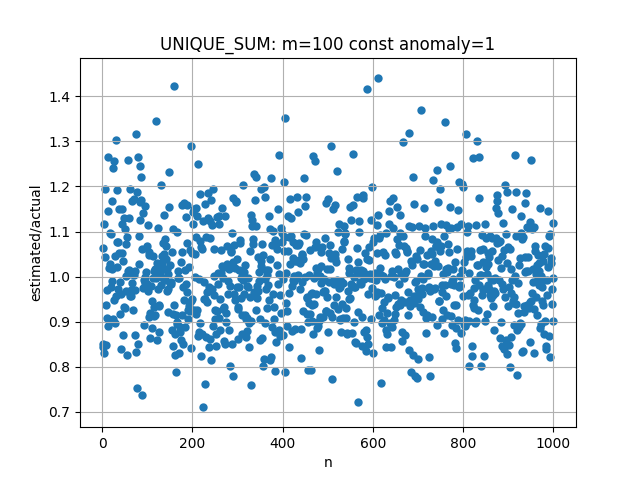
\includegraphics[width=\linewidth]{sum/zad1_const_1.png}
            \caption{$\lambda = \textnormal{const}$, $1\%$ wartości odstających}
        \end{subfigure}
        \begin{subfigure}{0.6\textwidth}
            \centering
            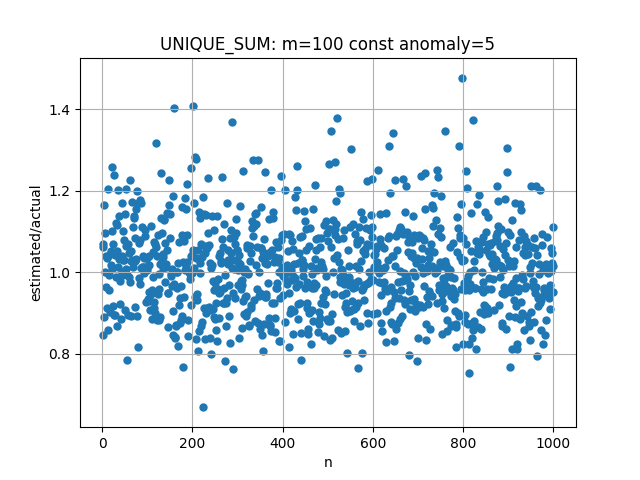
\includegraphics[width=\linewidth]{sum/zad1_const_5.png}
            \caption{$\lambda = \textnormal{const}$, $5\%$ wartości odstających}
        \end{subfigure}
        \begin{subfigure}{0.6\textwidth}
            \centering
            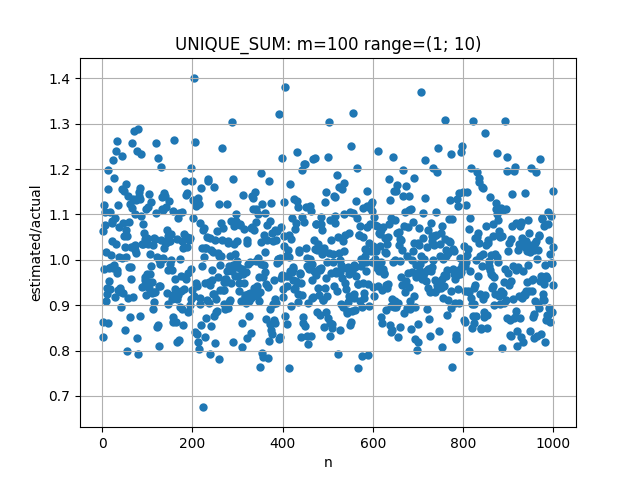
\includegraphics[width=\linewidth]{sum/zad1_range_1_10.png}
            \caption{$\lambda \in [1, 10]$}
        \end{subfigure}
        \begin{subfigure}{0.6\textwidth}
            \centering
            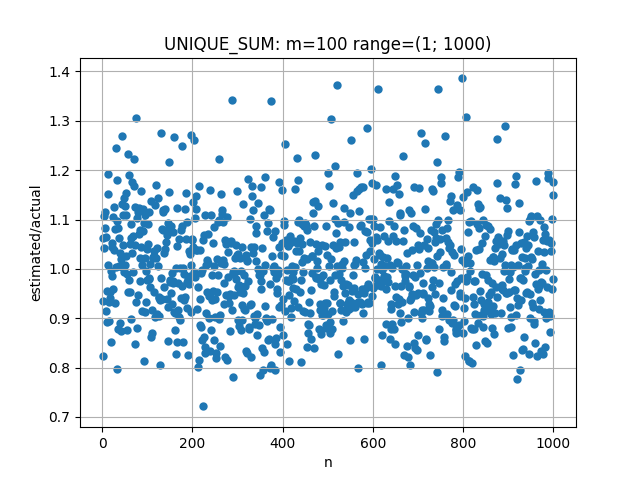
\includegraphics[width=\linewidth]{sum/zad1_range_1_1000.png}
            \caption{$\lambda \in [1, 1000]$}
        \end{subfigure}
        \begin{subfigure}{0.6\textwidth}
            \centering
            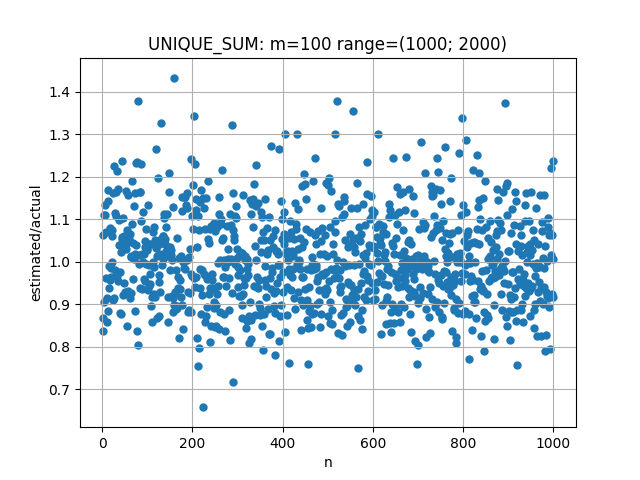
\includegraphics[width=\linewidth]{sum/zad1_range_1000_2000.png}
            \caption{$\lambda \in [1000, 2000]$}
        \end{subfigure}
        \caption{Wykresy dla $m = 100$ i funkcji haszującej $h = hash1$}
    \end{figure}

    Dokładność estymowanej sumy jest podobna, niezależnie od tego w jaki sposób wybrane 
    zostały wartości $\lambda$ elementów zbioru.

    \subsubsection{Nierówność Czebyszewa}

    $\alpha = 0.5\%$:

    \begin{figure}[H]
        \begin{subfigure}{0.6\textwidth}
            \centering
            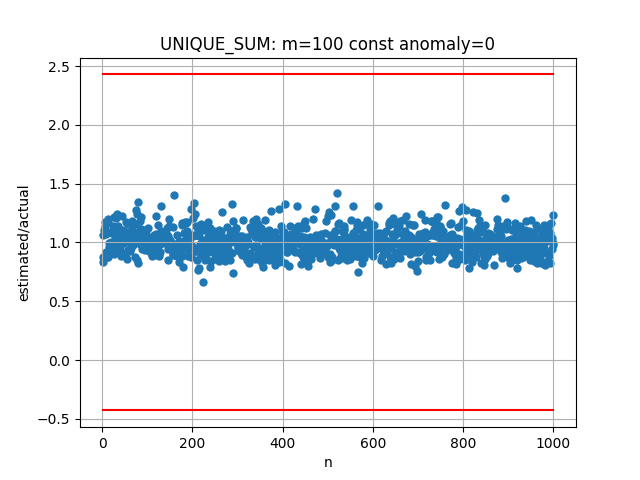
\includegraphics[width=\linewidth]{sum/zad1_const_0_cheb_05.png}
            \caption{$\lambda = \textnormal{const}$}
        \end{subfigure}
        \begin{subfigure}{0.6\textwidth}
            \centering
            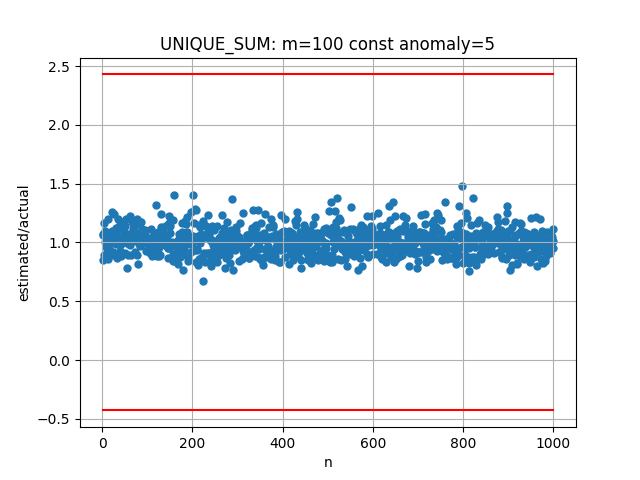
\includegraphics[width=\linewidth]{sum/zad1_const_5_cheb_05.png}
            \caption{$\lambda = \textnormal{const}$, $5\%$ wartości odstających}
        \end{subfigure}
        \begin{subfigure}{0.6\textwidth}
            \centering
            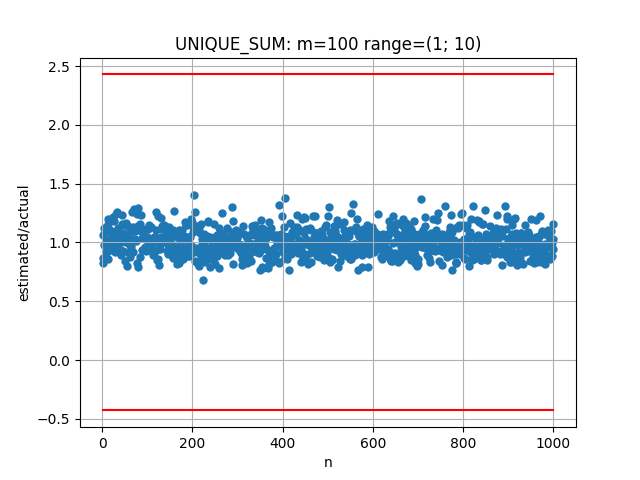
\includegraphics[width=\linewidth]{sum/zad1_range_1_10_cheb_05.png}
            \caption{$\lambda \in [1, 10]$}
        \end{subfigure}
        \begin{subfigure}{0.6\textwidth}
            \centering
            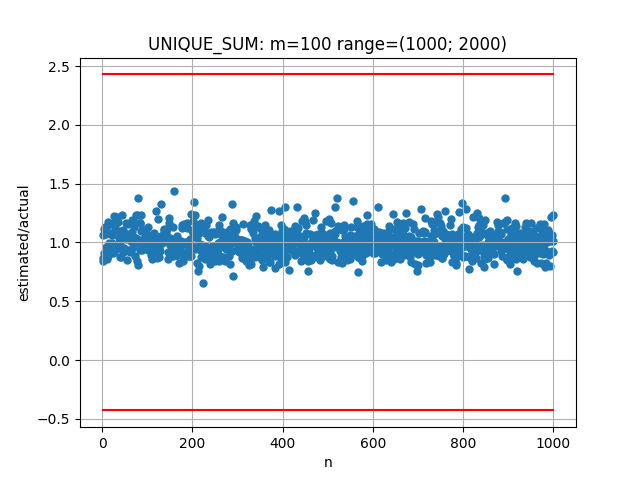
\includegraphics[width=\linewidth]{sum/zad1_range_1000_2000_cheb_05.png}
            \caption{$\lambda \in [1000, 2000]$}
        \end{subfigure}
        \caption{Wykresy dla $m = 100$ i funkcji haszującej $h = hash1$ (ograniczenie z nierówności Czebyszewa dla parametru $\alpha = 0.5\%$)}
    \end{figure}

    $\alpha = 1\%$:
            
    \begin{figure}[H]
        \begin{subfigure}{0.6\textwidth}
            \centering
            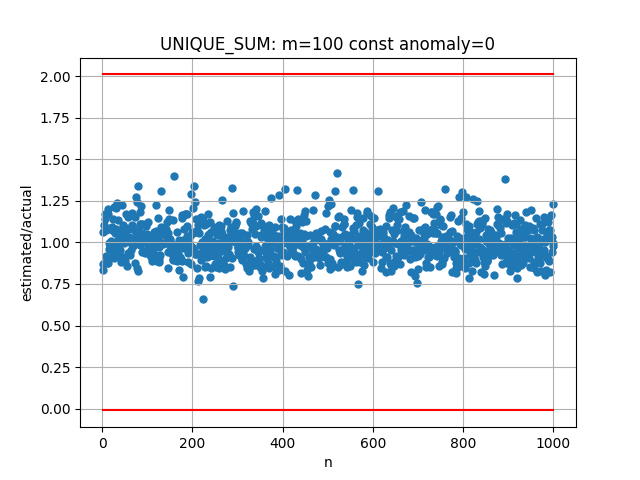
\includegraphics[width=\linewidth]{sum/zad1_const_0_cheb_1.png}
            \caption{$\lambda = \textnormal{const}$}
        \end{subfigure}
        \begin{subfigure}{0.6\textwidth}
            \centering
            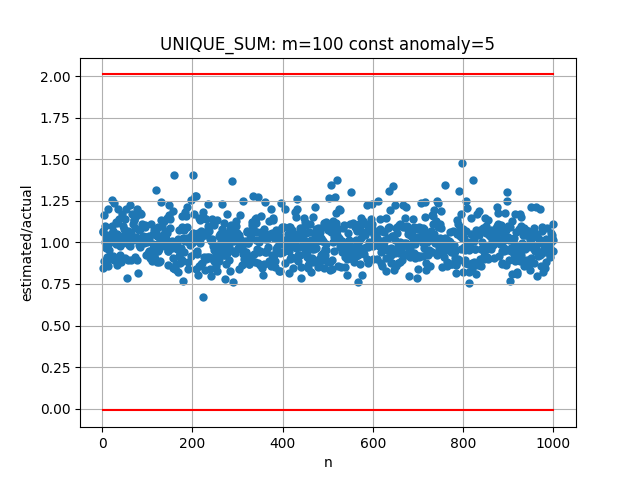
\includegraphics[width=\linewidth]{sum/zad1_const_5_cheb_1.png}
            \caption{$\lambda = \textnormal{const}$, $5\%$ wartości odstających}
        \end{subfigure}
        \begin{subfigure}{0.6\textwidth}
            \centering
            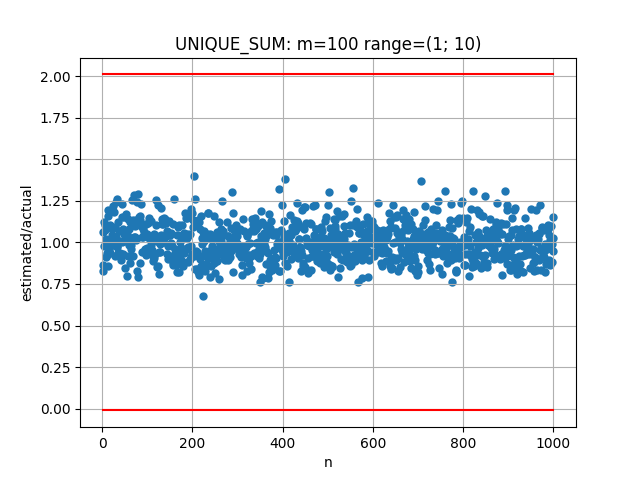
\includegraphics[width=\linewidth]{sum/zad1_range_1_10_cheb_1.png}
            \caption{$\lambda \in [1, 10]$}
        \end{subfigure}
        \begin{subfigure}{0.6\textwidth}
            \centering
            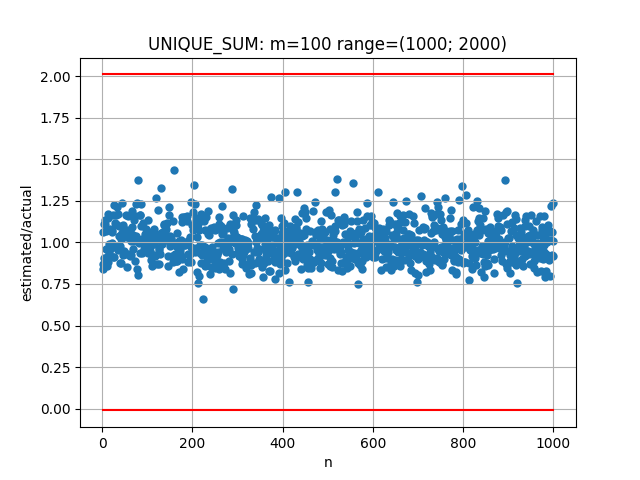
\includegraphics[width=\linewidth]{sum/zad1_range_1000_2000_cheb_1.png}
            \caption{$\lambda \in [1000, 2000]$}
        \end{subfigure}
        \caption{Wykresy dla $m = 100$ i funkcji haszującej $h = hash1$ (ograniczenie z nierówności Czebyszewa dla parametru $\alpha = 1\%$)}
    \end{figure}

    $\alpha = 5\%$:
        
    \begin{figure}[H]
        \begin{subfigure}{0.6\textwidth}
            \centering
            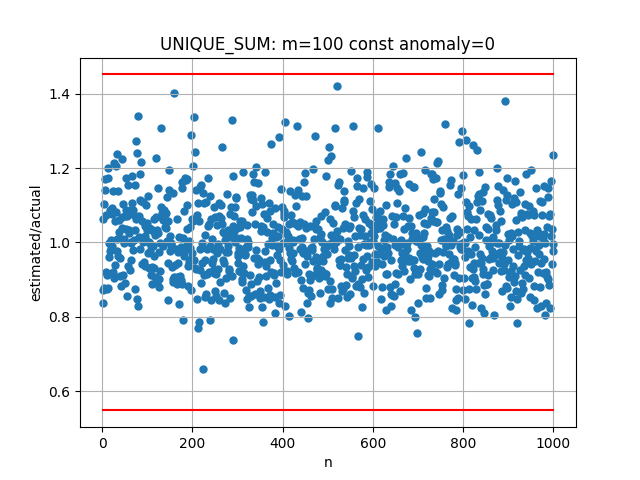
\includegraphics[width=\linewidth]{sum/zad1_const_0_cheb_5.png}
            \caption{$\lambda = \textnormal{const}$}
        \end{subfigure}
        \begin{subfigure}{0.6\textwidth}
            \centering
            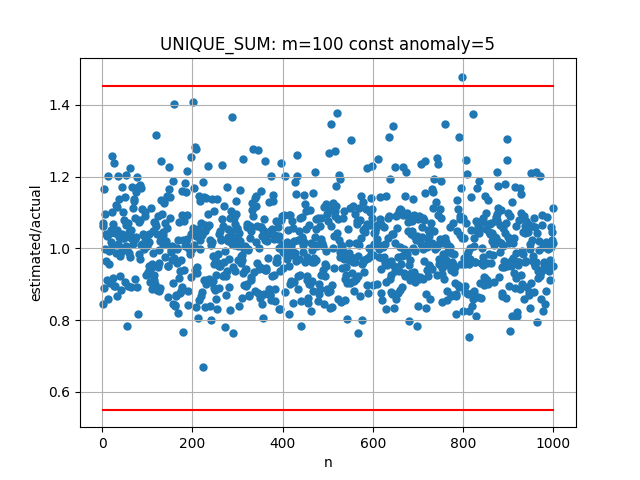
\includegraphics[width=\linewidth]{sum/zad1_const_5_cheb_5.png}
            \caption{$\lambda = \textnormal{const}$, $5\%$ wartości odstających}
        \end{subfigure}
        \begin{subfigure}{0.6\textwidth}
            \centering
            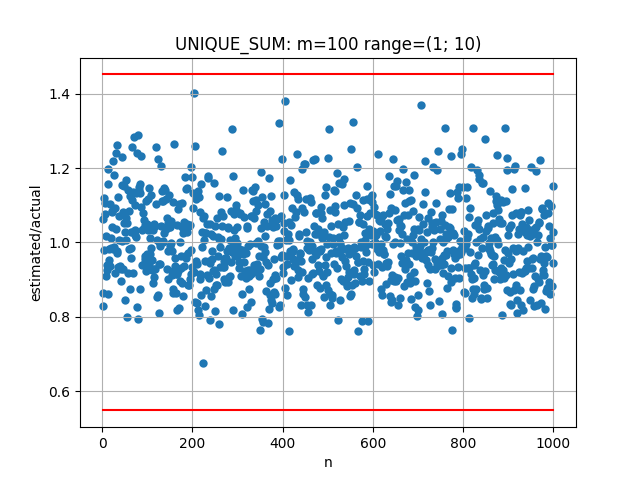
\includegraphics[width=\linewidth]{sum/zad1_range_1_10_cheb_5.png}
            \caption{$\lambda \in [1, 10]$}
        \end{subfigure}
        \begin{subfigure}{0.6\textwidth}
            \centering
            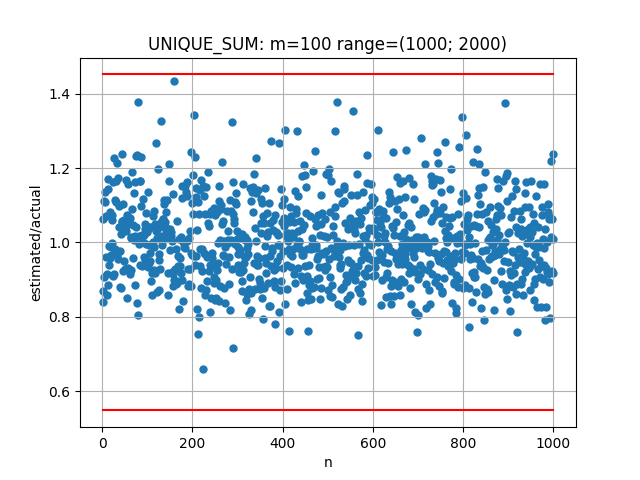
\includegraphics[width=\linewidth]{sum/zad1_range_1000_2000_cheb_5.png}
            \caption{$\lambda \in [1000, 2000]$}
        \end{subfigure}
        \caption{Wykresy dla $m = 100$ i funkcji haszującej $h = hash1$ (ograniczenie z nierówności Czebyszewa dla parametru $\alpha = 5\%$)}
    \end{figure}


	\section{Zadanie 10}
	\subsection{Opis zadania}
        Zaproponuj i przetestuj procedurę, która umożliwi w oszacowanie średniej wartości unikalnych elementów 
        $$\frac{\lambda_1 + \lambda_2 + \dots + \lambda_n}{n}$$ w ramach jednego przebiegu po multizbiorze.

    
    \subsection{Rozwiązanie}

    Proponowany algorytm jest modyfikacją algorytmu UNIQUE\_SUM. Modyfikacja polega na tym, że oprócz tablicy 
    $M$ wprowadzamy tablicę $N$, która będzie służyć estymacji liczby wszystkich unikalnych elementów multizbioru. 
    Podobnie jak w przypadku tablicy zawartości tablicy $M$, zawartość $N$ jest uaktualniana dla każdego elementu 
    multizbioru w sposób przedstawiony na poniższym pseudokodzie:
    \\

    \begin{pseudokod}[H]
        \caption{UniqueAvg($\mathfrak{M}, h, m$)}
        \SetKwInOut{Input}{Input}
        \SetKwInOut{Output}{Output}
        \Input{$\mathfrak{M}$, $h$, $m$}
        \Output{$avg$ - średnia wartość unikalnych elementów}
        \BlankLine
        Set each of $m$ positions of $M$ and $N$ to $\infty$;
        \BlankLine
        \For{$(i, \lambda_i) \in \mathfrak{M}$} {
            \For{$k \in \{1,2,\dots,m\}$}{
                $u \gets h(i ^\frown k)$\;
                $M[k] \gets \min(M[k], -\frac{\ln{u}}{\lambda_i})$\;
                $N[k] \gets \min(N[k], -\frac{\ln{u}}{1})$\;
            }
        }
        $\bar{\Lambda} \gets \frac{m-1}{\sum_{k=1}^{m}M[k]}$\;
        $\bar{c} \gets \frac{m-1}{\sum_{k=1}^{m}N[k]}$\;

        \Return{$avg = \frac{\bar{\Lambda}}{\bar{c}}$}
    \end{pseudokod}

    \subsubsection{Wyniki dla różnych wartości $\lambda$}

    \begin{figure}[H]
        \begin{subfigure}{0.6\textwidth}
            \centering
            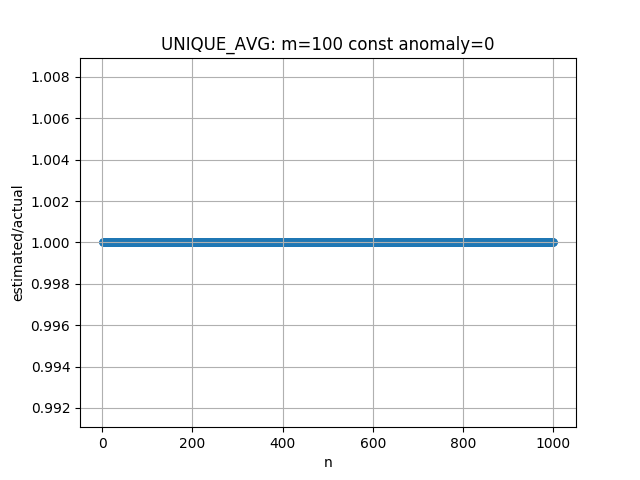
\includegraphics[width=\linewidth]{avg/zad1_const_0.png}
            \caption{$\lambda = \textnormal{const}$}
        \end{subfigure}
        \begin{subfigure}{0.6\textwidth}
            \centering
            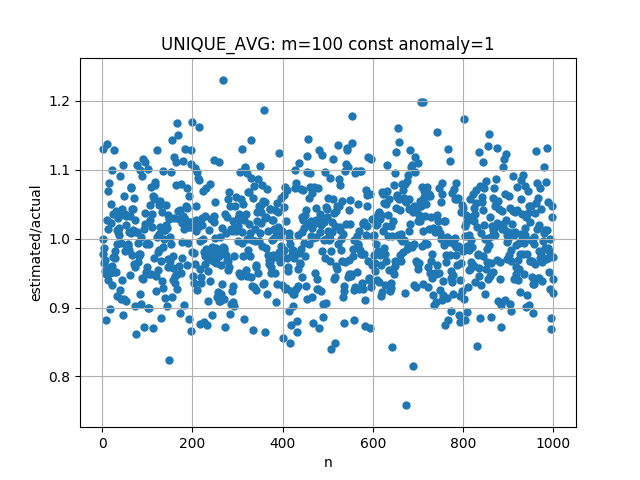
\includegraphics[width=\linewidth]{avg/zad1_const_1.png}
            \caption{$\lambda = \textnormal{const}$, $1\%$ wartości odstających}
        \end{subfigure}
        \begin{subfigure}{0.6\textwidth}
            \centering
            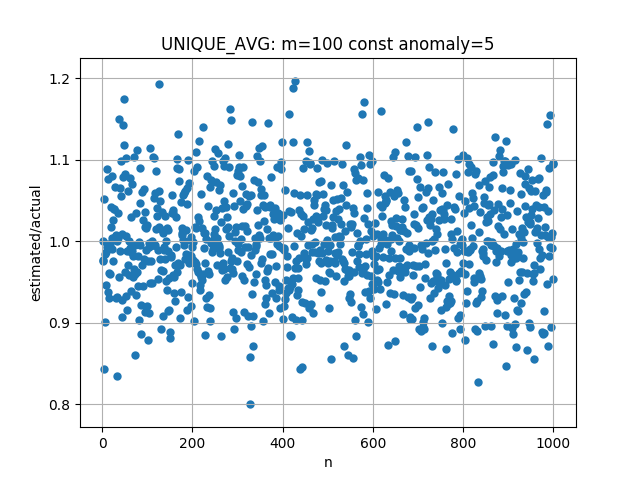
\includegraphics[width=\linewidth]{avg/zad1_const_5.png}
            \caption{$\lambda = \textnormal{const}$, $5\%$ wartości odstających}
        \end{subfigure}
        \begin{subfigure}{0.6\textwidth}
            \centering
            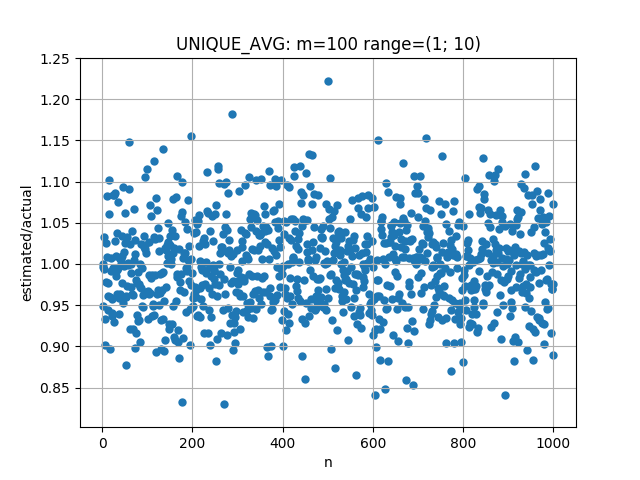
\includegraphics[width=\linewidth]{avg/zad1_range_1_10.png}
            \caption{$\lambda \in [1, 10]$}
        \end{subfigure}
        \begin{subfigure}{0.6\textwidth}
            \centering
            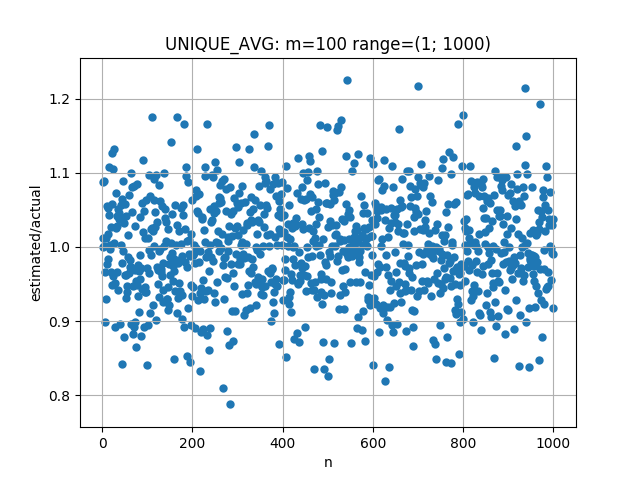
\includegraphics[width=\linewidth]{avg/zad1_range_1_1000.png}
            \caption{$\lambda \in [1, 1000]$}
        \end{subfigure}
        \begin{subfigure}{0.6\textwidth}
            \centering
            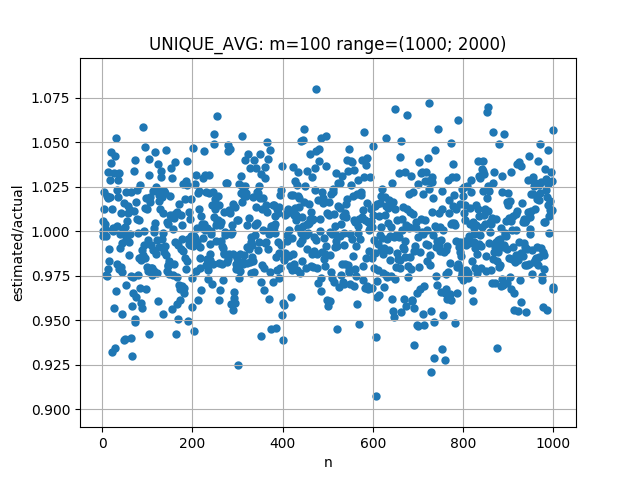
\includegraphics[width=\linewidth]{avg/zad1_range_1000_2000.png}
            \caption{$\lambda \in [1000, 2000]$}
        \end{subfigure}
        \caption{Wykresy dla $m = 100$ i funkcji haszującej $h = hash1$}
    \end{figure}


\end{document}